\documentclass[border=3pt]{standalone}
% Preâmbulo compartilhado pelos diagramas TikZ da aula 10 (Localização de Markov e Gaussiana)
\usepackage[T1]{fontenc}
\usepackage[utf8]{inputenc}
\usepackage{lmodern}
\usepackage{amsmath}
\usepackage{xcolor}
\usepackage{tikz}
\usetikzlibrary{arrows.meta,angles,quotes,decorations.pathmorphing,calc,
                positioning,shapes.geometric,shapes.misc,backgrounds,fit,
                math}

% Paleta (mesma dos SVGs originais)
\definecolor{dblue}{HTML}{2A5B8C}
\definecolor{dorange}{HTML}{B3541E}
\definecolor{dgreen}{HTML}{4A7C59}
\definecolor{dred}{HTML}{9C4B4B}
\definecolor{dcream}{HTML}{F4F1EA}
\definecolor{dshade}{HTML}{DDD7C9}

% Função gaussiana (não normalizada por padrão de escala visual)
\pgfmathdeclarefunction{gauss}{3}{%
  \pgfmathparse{1/(#3*sqrt(2*pi))*exp(-((#1-#2)^2)/(2*#3^2))}%
}

% Estilos comuns (prefixo d... para não colidir com chaves internas do pgf)
\tikzset{
  >={Stealth[length=2mm]},
  dguide/.style={gray!55, dashed, line width=0.4pt},
  daxis/.style={gray!60, line width=0.7pt, ->},
  dbody/.style={fill=black!3, draw=black!80, line width=1pt},
  dacc/.style={draw=dblue, line width=1pt},
  dlbl/.style={black!55, font=\small},
  dsub/.style={black!45, font=\footnotesize},
  dstate/.style={circle, draw=black!80, fill=dcream, line width=1pt,
                 minimum size=17mm, font=\large, inner sep=1pt},
  dobs/.style={circle, draw=black!80, fill=dshade, line width=1pt,
               minimum size=14mm, font=\large, inner sep=1pt},
  dbox/.style={rounded corners=2pt, draw=black!80, fill=dcream, line width=1pt,
               align=center, inner sep=6pt},
  dop/.style={circle, draw=black!80, fill=white, line width=1pt,
              minimum size=6mm, inner sep=0pt, font=\small},
  dtrans/.style={->, dblue, line width=1pt},
  dmeas/.style={->, dorange, line width=1pt},
  dcurve/.style={line width=1pt, dblue},
  dcurveb/.style={line width=1.4pt, dorange},
}

\usetikzlibrary{shapes.callouts}
\begin{document}
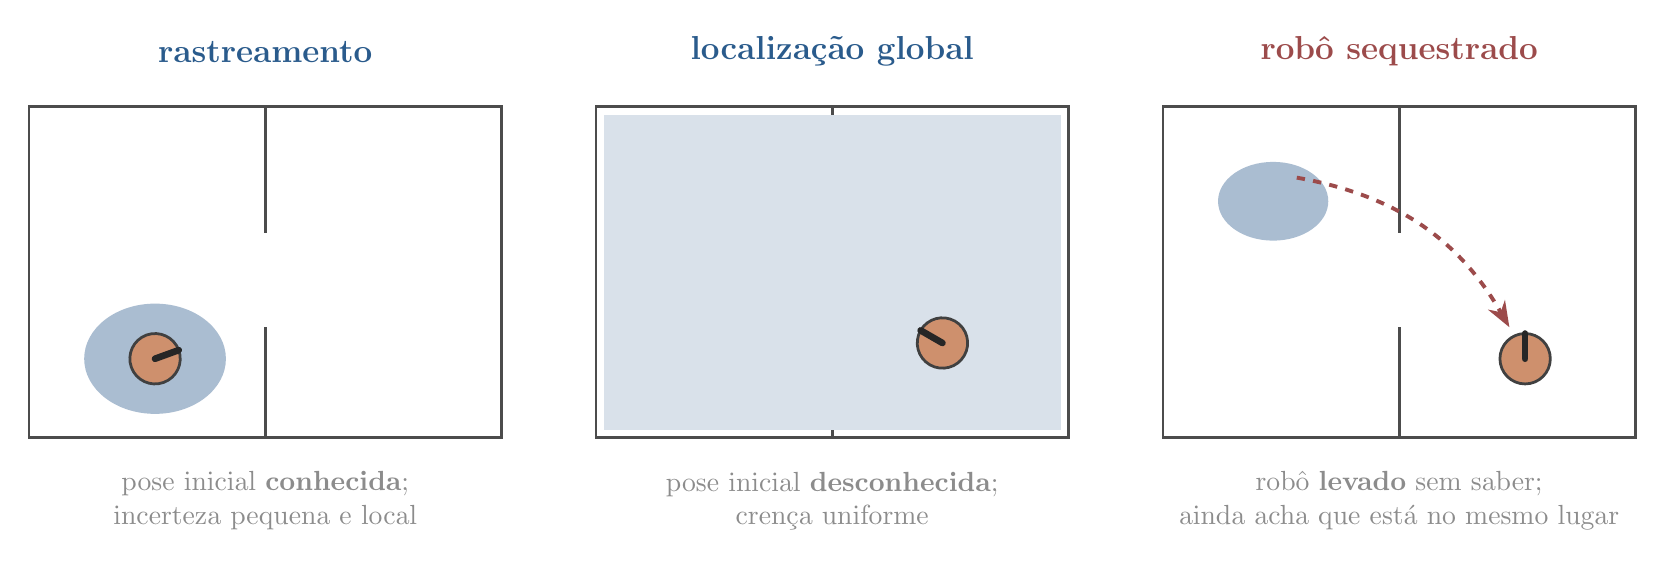
\begin{tikzpicture}[x=1cm,y=1cm,bal/.style={rectangle callout, rounded corners=7pt, draw=black!75, fill=white, line width=1pt, align=center, font=\normalsize, inner sep=5pt}]
  \newcommand{\robo}[3]{\begin{scope}[shift={(#1,#2)}, rotate=#3]\draw[black!75, fill=dorange!65, line width=1pt] (0,0) circle (0.32); \draw[black!85, line width=2.4pt, line cap=round] (0,0) -- (0.32,0);\end{scope}}

  \newcommand{\planta}[1]{\draw[black!70, fill=white, line width=1pt] (#1,0) rectangle (#1+6,4.2); \draw[black!70, line width=1pt] (#1+3,0) -- (#1+3,1.4) (#1+3,2.6) -- (#1+3,4.2);}
  \begin{scope}
    \planta{0} \fill[dblue!40] (1.6,1.0) ellipse (0.9 and 0.7); \robo{1.6}{1.0}{20}
    \node[font=\bfseries\large, dblue] at (3,4.9) {rastreamento};
    \node[dsub, font=\normalsize, align=center] at (3,-0.8) {pose inicial \textbf{conhecida};\\ incerteza pequena e local};
  \end{scope}
  \begin{scope}[shift={(7.2,0)}]
    \planta{0} \fill[dblue!18] (0.1,0.1) rectangle (5.9,4.1); \robo{4.4}{1.2}{150}
    \node[font=\bfseries\large, dblue] at (3,4.9) {localização global};
    \node[dsub, font=\normalsize, align=center] at (3,-0.8) {pose inicial \textbf{desconhecida};\\ crença uniforme};
  \end{scope}
  \begin{scope}[shift={(14.4,0)}]
    \planta{0} \fill[dblue!40] (1.4,3.0) ellipse (0.7 and 0.5); \robo{4.6}{1.0}{90}
    \draw[dred, dashed, line width=1.4pt, -{Stealth}] (1.7,3.3) to[bend left=25] (4.4,1.4);
    \node[font=\bfseries\large, dred] at (3,4.9) {robô sequestrado};
    \node[dsub, font=\normalsize, align=center] at (3,-0.8) {robô \textbf{levado} sem saber;\\ ainda acha que está no mesmo lugar};
  \end{scope}
\end{tikzpicture}
\end{document}
